\documentclass[11pt,letterpaper]{article}
\usepackage[margin=0.85in,headheight=14pt]{geometry}
\usepackage{amsmath,amssymb}
\usepackage{enumitem}
\usepackage{fancyhdr}
\usepackage{lmodern}
\usepackage[T1]{fontenc}
\usepackage[dvipsnames]{xcolor}
\usepackage[most]{tcolorbox}
\usepackage{listings}
\usepackage{pgfplots}
\usepgfplotslibrary{groupplots,fillbetween}
\usetikzlibrary{arrows.meta,positioning,shapes.geometric}
\pgfplotsset{
  compat=1.18,
  every axis/.append style={grid=major, grid style={gray!25}, tick label style={font=\footnotesize},
    label style={font=\small}, title style={font=\small}, legend style={font=\scriptsize}},
}
\definecolor{cA}{HTML}{1F77B4}
\definecolor{cB}{HTML}{FF7F0E}
\definecolor{cC}{HTML}{2CA02C}
\definecolor{cD}{HTML}{D62728}
\definecolor{cE}{HTML}{9467BD}
\definecolor{cF}{HTML}{8C564B}

\pagestyle{fancy}
\fancyhf{}
\lhead{SYDE 556/750 \qquad Ramp practice}
\rhead{Solutions}
\cfoot{\thepage}
\renewcommand{\headrulewidth}{0pt}

\setlength{\parindent}{0pt}
\setlength{\parskip}{4pt}

\newcommand{\T}{\mathsf{T}}
\newcommand{\tin}{\tau_{\mathrm{in}}}
\newcommand{\ans}[1]{\par\vspace{4pt}{\bfseries #1}\quad}

\newtcolorbox{result}{colback=Green!6,colframe=Green!50!black,boxrule=0.5pt,left=4pt,right=4pt,top=2pt,bottom=2pt,arc=1pt}
\newtcolorbox{trap}{colback=red!4,colframe=red!50!black,boxrule=0.4pt,left=4pt,right=4pt,top=2pt,bottom=2pt,arc=1pt,fonttitle=\bfseries\small,title=Where marks are usually lost}

\lstset{basicstyle=\ttfamily\small, columns=fullflexible, keepspaces=true, frame=single, rulecolor=\color{gray!50}}

\tikzset{box/.style={draw, thick, rounded corners, minimum height=0.8cm, minimum width=1.3cm, align=center, font=\small},
  ens/.style={draw, thick, ellipse, minimum height=0.9cm, minimum width=1.6cm, align=center, font=\small},
  lab/.style={font=\scriptsize, align=center}}

\begin{document}

\begin{center}
{\Large\bfseries Ramp practice solutions}\\[2pt]
{\large Decision making, the LMU, learning, and analysing representation}\\[4pt]
Open a solution only after attempting that question. Each green box is the result.\\
Simulated traces come from \texttt{pn4\_data/make\_data.py} (Nengo~4.1, seed $556$, the PN4 settings).
\end{center}

%=====================================================================
\part*{Part A}
%=====================================================================

\section{The PN4 accumulator is an integrator with a large input gain}

\ans{Q1}
$A' = 1 \Rightarrow A = (A' - 1)/\tau = 0$, and $B' = 1 \Rightarrow B = 1/\tau = 10\,\mathrm{s^{-1}}$. So $\dot x = 10u$, and a constant $u$ gives a ramp of slope $10u$. The input-synapse mismatch adds an offset of $(1 - \tin/\tau)u = 0.95u$ within about $3\tin = 15\,\mathrm{ms}$:
\[
x(t) \approx 10u\,t + 0.95u \qquad (\text{until saturation}).
\]
\begin{center}
\renewcommand{\arraystretch}{1.15}
\begin{tabular}{c|c|c|c|c|c}
$u$ & slope (s$^{-1}$) & offset & $|x| = 0.9$, ideal & $|x| = 0.9$, with offset & Nengo \\ \hline
$\pm0.2$ & $\pm2$ & $\pm0.19$ & $0.45\,\mathrm{s}$ & $(0.9 - 0.19)/2 = 0.355\,\mathrm{s}$ & $0.36$, $0.37\,\mathrm{s}$\\
$\pm0.1$ & $\pm1$ & $\pm0.095$ & $0.90\,\mathrm{s}$ & $(0.9 - 0.095)/1 = 0.805\,\mathrm{s}$ & $0.81$, $0.82\,\mathrm{s}$
\end{tabular}
\end{center}
Each trace jumps by its offset, ramps, and then flattens just beyond $\pm1$ (Section~2). The $\pm$ pairs are mirror images.
\begin{center}
\begin{tikzpicture}
\begin{axis}[width=0.9\textwidth, height=6cm, xmin=0, xmax=2, ymin=-1.25, ymax=1.25,
  xlabel={$t$ (s)}, ylabel={accumulator $x$}, legend style={at={(0.5,1.03)}, anchor=south, legend columns=5},
  legend cell align=left]
  \addplot[cA, very thick] table[x=t, y=u02] {pn4_data/acc_clean.dat};
  \addplot[cB, very thick] table[x=t, y=u01] {pn4_data/acc_clean.dat};
  \addplot[cC, very thick] table[x=t, y=um01] {pn4_data/acc_clean.dat};
  \addplot[cD, very thick] table[x=t, y=um02] {pn4_data/acc_clean.dat};
  \addplot[black, dashed, domain=0:0.405, samples=2] {2*x+0.19};
  \addplot[black, dashed, domain=0:0.905, samples=2, forget plot] {x+0.095};
  \addplot[black, dashed, domain=0:0.905, samples=2, forget plot] {-x-0.095};
  \addplot[black, dashed, domain=0:0.405, samples=2, forget plot] {-2*x-0.19};
  \legend{$u = 0.2$, $u = 0.1$, $u = -0.1$, $u = -0.2$, prediction $10ut + 0.95u$}
  \addplot[gray, dotted, thick, domain=0:2, samples=2, forget plot] {0.9};
  \addplot[gray, dotted, thick, domain=0:2, samples=2, forget plot] {-0.9};
  \node[font=\scriptsize, anchor=south west, fill=white, inner sep=1pt] at (axis cs:0.02,0.92) {$0.9$};
\end{axis}
\end{tikzpicture}
\end{center}

\ans{Q2}
\textbf{Input \texttt{transform=tau}.} Now $B' = 0.1$, so $B = 1\,\mathrm{s^{-1}}$ and the slope for $u = 0.1$ is $0.1\,\mathrm{s^{-1}}$, ten times slower. The offset is $(1 - \tin/\tau)B'u = 0.95 \times 0.01 \approx 0.01$. At $t = 2\,\mathrm{s}$, $x \approx 0.21$. It never reaches $0.9$ in the run. There is nothing wrong with \texttt{transform=tau}; it builds $\dot x = u$ rather than $\dot x = 10u$.

\textbf{Recurrent synapse $10\,\mathrm{ms}$, \texttt{transform=1} on both.} $A' = 1$ still gives an integrator, but now $B = B'/\tau = 1/0.01 = 100\,\mathrm{s^{-1}}$. The offset is $(1 - 0.005/0.01)u = 0.5u = 0.05$, so $x \approx 10t + 0.05$ reaches $0.9$ at about $0.085\,\mathrm{s}$. The $5\,\mathrm{ms}$ input filter is no longer short compared with this, so treat it as rough. A $10\,\mathrm{ms}$ loop also holds its value less well, because distortion makes the state drift with time constants of order $\tau$ (PN3).

With the input transform fixed, the recurrent synapse sets the rate of accumulation: $B = B'/\tau$.
\begin{result}
Slope $10u$ and offset $0.95u$. $|x| = 0.9$ at $0.355\,\mathrm{s}$ ($|u| = 0.2$) and $0.805\,\mathrm{s}$ ($|u| = 0.1$). With \texttt{transform=tau}: $\dot x = u$, reaching only about $0.21$ in $2\,\mathrm{s}$. With a $10\,\mathrm{ms}$ recurrence: $\dot x = 100u$, reaching $0.9$ at about $0.085\,\mathrm{s}$.
\end{result}

\section{Why the accumulator stops at the radius}

\ans{Q1}
The ideal computation is $x(t) = \frac{1}{\tau}\int_0^t u(t')\,dt'$: the output is the running integral of the evidence, scaled by $1/\tau$. Here that is $10\int u$.

The neural recurrence decodes $\hat f(x)$, not $x$, so $\tau\dot x = \hat f(x) - x + u$. Inside $[-1, 1]$, $\hat f(x) - x \approx 0$ and $x$ ramps at $u/\tau$. Beyond $+1$ the positive-encoder neurons are near their maximum rates and $\hat f$ falls below $x$, so $\hat f(x) - x$ becomes increasingly negative. The state stops where $\hat f(x) - x = -u$. A larger $u$ needs a more negative $\hat f(x) - x$, which only happens further out, so the $u = 0.2$ trace stops higher ($1.14$ against $1.08$ in Nengo). The equilibrium is stable because $\tau\dot x$ crosses zero going downward there.
\begin{center}
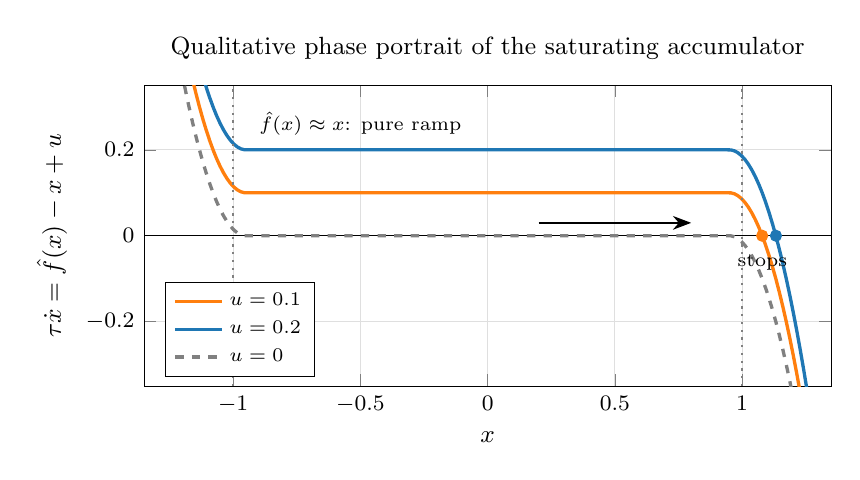
\begin{tikzpicture}[declare function={g(\x) = -6*(\x > 0.95)*(\x - 0.95)^2 + 6*(\x < -0.95)*(\x + 0.95)^2;}]
\begin{axis}[width=0.85\textwidth, height=5.4cm, xmin=-1.35, xmax=1.35, ymin=-0.35, ymax=0.35,
  xlabel={$x$}, ylabel={$\tau\dot x = \hat f(x) - x + u$}, legend pos=south west, legend cell align=left,
  title={Qualitative phase portrait of the saturating accumulator}]
  \addplot[black, domain=-1.35:1.35, samples=2, forget plot] {0};
  \addplot[cB, very thick, domain=-1.35:1.35, samples=200] {0.1 + g(x)};
  \addplot[cA, very thick, domain=-1.35:1.35, samples=200] {0.2 + g(x)};
  \addplot[gray, very thick, dashed, domain=-1.35:1.35, samples=200] {g(x)};
  \legend{$u = 0.1$, $u = 0.2$, $u = 0$}
  \addplot[only marks, mark=*, cB] coordinates {(1.079,0)};
  \addplot[only marks, mark=*, cA] coordinates {(1.133,0)};
  \draw[-{Stealth}, thick] (axis cs:0.2,0.03) -- (axis cs:0.8,0.03);
  \node[font=\scriptsize, anchor=north] at (axis cs:1.08,-0.02) {stops};
  \draw[gray, dotted, thick] (axis cs:1,-0.35) -- (axis cs:1,0.35);
  \draw[gray, dotted, thick] (axis cs:-1,-0.35) -- (axis cs:-1,0.35);
  \node[font=\scriptsize, anchor=south] at (axis cs:-0.5,0.21) {$\hat f(x) \approx x$: pure ramp};
\end{axis}
\end{tikzpicture}
\end{center}
\ans{Q2}
Ideally, $x$ is $\int u/\tau$ and keeps climbing, reaching $1.5 + 0.095$ at $t = 1.5\,\mathrm{s}$. When the input is removed it holds $1.5$. The neural state cannot follow. When the input goes off, the $+u$ term and the $0.95u$ offset both vanish, the equilibrium moves back to where $\hat f(x) = x$, near the radius, and the state drops slightly to about $1$. It then holds there, with the slow drift of a real integrator.

With radius $2$, the dynamics inside the range are unchanged, so $0.9$ is still reached at about $0.805\,\mathrm{s}$. The trace then keeps ramping to about $2$ (near $t \approx 1.9\,\mathrm{s}$) before it saturates. The cost: every decoding error is multiplied by the radius (Test~3), so the state is twice as noisy and drifts more.
\begin{result}
$x = \frac1\tau\int u$ until saturation. It stops just beyond $\pm1$, where $\hat f(x) - x = -u$, and stronger inputs stop a little further out. With radius $2$ the threshold time is unchanged and the trace saturates near $2$, with about twice the error.
\end{result}

\section{Noise turns accumulation into a random walk}

\ans{Q1}
Mean $= 10u\,t$ and standard deviation $= 0.3\sqrt{t}$.
\begin{center}
\renewcommand{\arraystretch}{1.15}
\begin{tabular}{c|c|c|c|c}
$u$ & mean at $0.5\,\mathrm s$ & s.d.\ at $0.5\,\mathrm s$ & mean / s.d. & $P(x < 0)$ \\ \hline
$0.1$ & $0.5$ & $0.3\sqrt{0.5} \approx 0.21$ & $2.36$ & $\approx 1\%$\\
$0.05$ & $0.25$ & $0.21$ & $1.18$ & $\approx 12\%$
\end{tabular}
\end{center}
The weaker input is about ten times more likely to be on the wrong side. The reliability ratio is $\text{mean}/\text{s.d.} = 10u\sqrt t/\sigma$. Halving $u$ must be paid for by doubling $\sqrt t$, so $u = 0.05$ needs $t = 2\,\mathrm{s}$, four times longer, to match $u = 0.1$ at $0.5\,\mathrm{s}$. This is the speed--accuracy trade-off.
\begin{center}
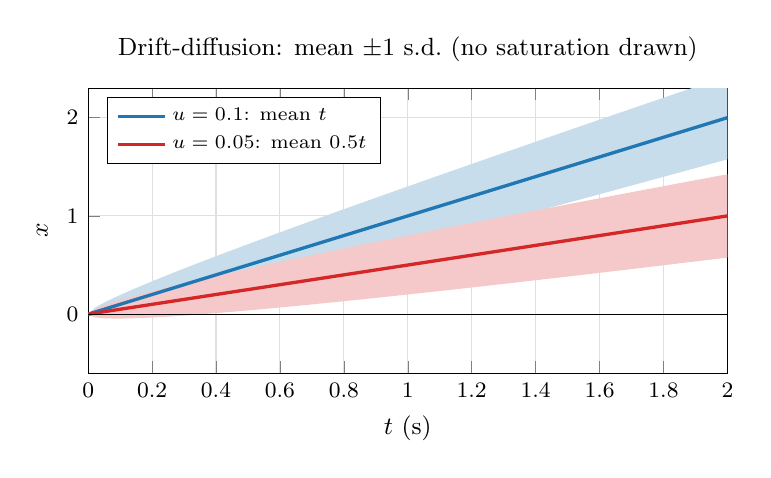
\begin{tikzpicture}
\begin{axis}[width=0.8\textwidth, height=5.2cm, xmin=0, xmax=2, ymin=-0.6, ymax=2.3,
  xlabel={$t$ (s)}, ylabel={$x$}, legend pos=north west, legend cell align=left,
  title={Drift-diffusion: mean $\pm 1$ s.d.\ (no saturation drawn)}]
  \addplot[name path=a1, draw=none, domain=0:2, samples=100, forget plot] {x + 0.3*sqrt(x)};
  \addplot[name path=a2, draw=none, domain=0:2, samples=100, forget plot] {x - 0.3*sqrt(x)};
  \addplot[cA!25, forget plot] fill between[of=a1 and a2];
  \addplot[name path=b1, draw=none, domain=0:2, samples=100, forget plot] {0.5*x + 0.3*sqrt(x)};
  \addplot[name path=b2, draw=none, domain=0:2, samples=100, forget plot] {0.5*x - 0.3*sqrt(x)};
  \addplot[cD!25, forget plot] fill between[of=b1 and b2];
  \addplot[cA, very thick, domain=0:2, samples=2] {x};
  \addplot[cD, very thick, domain=0:2, samples=2] {0.5*x};
  \addplot[black, thin, domain=0:2, samples=2, forget plot] {0};
  \legend{$u = 0.1$: mean $t$, $u = 0.05$: mean $0.5t$}
\end{axis}
\end{tikzpicture}
\end{center}

\ans{Q2}
The decoders were solved for noise-free LIF tuning curves. Noise added to the input current changes each neuron's average rate as a function of $x$. A neuron near threshold now fires sometimes when it should be silent, and the curve is smoothed and its sharp onset is lost. Averaged over the noise, the population's effective tuning curves are no longer the ones the decoders were fitted to, so the decoded recurrent function $\hat f(x)$ is no longer $\approx x$. It is compressed toward zero at large $|x|$, so $\hat f(x) - x < 0$ there. That is a leak, $\tau\dot x = \hat f(x) - x + u$, which balances the small input at a value well inside the radius. Larger $|u|$ balances further out ($0.58$ and $-0.83$ for $|u| = 0.2$; $0.22$ and $-0.33$ for $|u| = 0.1$). On top of this, the noise adds the random walk, so the traces wander, and smaller inputs are hit hardest.
\begin{center}
\begin{tikzpicture}
\begin{axis}[width=0.85\textwidth, height=5.2cm, xmin=0, xmax=2, ymin=-1.25, ymax=1.25,
  xlabel={$t$ (s)}, ylabel={accumulator $x$}, legend pos=south west, legend cell align=left, legend columns=4,
  title={PN4 \S1c with \texttt{rms=10}: noisy, and leaky}]
  \addplot[cA, thick] table[x=t, y=u02] {pn4_data/acc_noise10.dat};
  \addplot[cB, thick] table[x=t, y=u01] {pn4_data/acc_noise10.dat};
  \addplot[cC, thick] table[x=t, y=um01] {pn4_data/acc_noise10.dat};
  \addplot[cD, thick] table[x=t, y=um02] {pn4_data/acc_noise10.dat};
  \legend{$0.2$, $0.1$, $-0.1$, $-0.2$}
\end{axis}
\end{tikzpicture}
\end{center}
With \texttt{rms=1} and \texttt{rms=3} the traces look like part (a) with visible jitter and a slightly slower ramp. At \texttt{rms=5} the weak inputs start to stall below $1$. At \texttt{rms=10} all four stall.
\begin{result}
Mean $10ut$, s.d.\ $0.3\sqrt t$. At $0.5\,\mathrm s$: $2.36$ s.d.\ ($u = 0.1$) against $1.18$ s.d.\ ($u = 0.05$); the weaker input needs $4\times$ the time. Strong current noise changes the effective tuning curves, so $\hat f(x) < x$ at large $|x|$: a leak, as well as a random walk.
\end{result}

\section{Decoding a step function from smooth tuning curves}

\ans{Q1}
From the plot: $\hat f(0.9) \approx 0.5$, $\hat f(1) \approx 0.77$, and the largest wiggle for $|x| < 0.8$ is about $0.14$.
\begin{itemize}[leftmargin=1.2em]
\item \textbf{At the jump} ($x = 0.9$): a sum of smooth curves cannot jump, so the least-squares fit passes through the midpoint and ramps over a width set by how fast the tuning curves bend, here about $0.1$--$0.2$.
\item \textbf{At the end} ($x = 1$): the fit has to rise from $0$ to $1$ over a very short stretch, and few neurons change their rate there. It undershoots the corner, much as a truncated series does.
\item \textbf{The wiggles}: forcing a flat $0$ over $[-0.9, 0.9]$ while also making the steep rise leaves ripples. The decoder trades error in the flat part for error at the jump.
\end{itemize}
Once decided, the accumulator sits at about $1.05$, beyond the range the decoder was fitted on. The decision population reports roughly $0.8$--$1$ (Nengo: about $1.0$ for $u = 0.2$, with noise \texttt{rms=3}). For $u = -0.1$ the noisy accumulator hovers near $-0.95$, right on the ramp, so the output only reaches about $-0.6$ and flickers. ``Snaps to $\pm1$'' is really ``ramps to most of $\pm1$''.

\ans{Q2}
With intercepts in $[0.4, 0.9]$, a neuron only fires when the input projected onto its encoder exceeds $0.4$. Before the decision, the input to the decision population is the wiggle, $|\hat f| \lesssim 0.15$ (plus spike noise), which is below every intercept. No neuron fires, so the decoded output is exactly $0$. Nengo gives a maximum of $|y| = 0.000$ before the decision, against $0.17$--$0.34$ with default intercepts. The population cannot represent values with $|y| < 0.4$: everything there reads as $0$. That does not matter here, because the only values that matter are $0$ and $\pm1$. The neurons' thresholds act as a dead zone, which is the clean-up we want.

\textbf{Combined 2-D ensemble.} The state $(x, y)$ can be as large as $(1.05, 1)$, so the norm reaches about $\sqrt2$. Use radius $\approx 1.5$. This makes every decoding error about $1.5\times$ larger, and 100 neurons spread over two dimensions represent each one worse than 50 neurons on one. So expect worse performance at 100 neurons, and most of it to come back at 500. The intercept trick fails because the same neurons must also represent the accumulator over its whole range, including small $x$. Intercepts above $0.4$ would make the population blind to every state with $|\langle e, (x, y)\rangle| < 0.4$, so the accumulator could not start from $0$.

\textbf{Biology.} Separate populations claim that the brain keeps ``evidence so far'' and ``choice'' in different neurons. One population claims mixed selectivity: single neurons respond to both. Test it by recording single neurons during the task and regressing each neuron's rate on both accumulated evidence and the eventual choice (one group of neurons per variable, or neurons tuned to both). Alternatively, silence one group and see whether the other variable survives.
\begin{result}
$\hat f(0.9) \approx 0.5$, $\hat f(1) \approx 0.77$, wiggles up to about $0.14$: smooth bases cannot jump. High intercepts give a dead zone, so the output is exactly $0$ until $|y| > 0.4$. A combined 2-D ensemble needs radius $\approx \sqrt2$, cannot use the trick, and claims mixed selectivity.
\end{result}

%=====================================================================
\part*{Part B}
%=====================================================================

\section{Functions as vectors: how many numbers does a window need?}

\ans{Q1}
$N = 2BT = 2 \times 5 \times 0.5 = 5$ numbers. Audio: $2 \times 20{,}000 \times 1 = 40{,}000$ samples. Real anti-aliasing filters cannot cut off sharply at $20\,\mathrm{kHz}$, so a little energy above $B$ leaks through. Sampling slightly faster than $2B$ leaves a guard band, so that energy does not alias back into the audible range.

\ans{Q2}
The fastest component is $B = 2\,\mathrm{Hz}$, so $2B\theta = 2 \times 2 \times 0.5 = 2$. That is a lower bound; the Pad\'e approximation is not a perfect sampler, so in practice more are needed ($q = 6$ works, and Section~9 shows $q = 4$--$8$ is best). White noise limited to $10\,\mathrm{Hz}$ over $\theta = 1\,\mathrm{s}$ needs $q \ge 20$.

One sample is not enough: both sines pass through every value in $[-1, 1]$, so any single number $u(t)$ is consistent with either frequency. Frequency is a property of how the signal changes over time, so it can only be read from a window.
\begin{result}
$5$ and $40{,}000$; guard band against aliasing. LMU lower bound $q \ge 2B\theta = 2$ (and $20$ for $10\,\mathrm{Hz}$ over $1\,\mathrm{s}$). One sample cannot reveal frequency.
\end{result}

\section{Basis coefficients when the basis is orthogonal but not orthonormal}

\ans{Q1}
$\int_0^1 1\cdot(2r - 1)\,dr = [r^2 - r]_0^1 = 0$, so they are orthogonal. $\int_0^1 (2r - 1)^2\,dr = \bigl[\tfrac{(2r - 1)^3}{6}\bigr]_0^1 = \tfrac16 + \tfrac16 = \tfrac13$.
\[
c_0 = 1\cdot\int_0^1 r\,dr = \tfrac12, \qquad c_1 = 3\int_0^1 r(2r - 1)\,dr = 3\bigl(\tfrac23 - \tfrac12\bigr) = \tfrac12.
\]
Check: $\tfrac12 + \tfrac12(2r - 1) = r$. Exact, since $r$ is a degree-1 polynomial.

\ans{Q2}
\[
c_0 = \int_0^1 r^2 = \tfrac13, \quad c_1 = 3\int_0^1 r^2(2r - 1) = 3\bigl(\tfrac12 - \tfrac13\bigr) = \tfrac12, \quad c_2 = 5\int_0^1 r^2(6r^2 - 6r + 1) = 5\bigl(\tfrac65 - \tfrac32 + \tfrac13\bigr) = \tfrac16.
\]
Check: $\tfrac13 + \tfrac12(2r - 1) + \tfrac16(6r^2 - 6r + 1) = r^2$. The $q = 2$ approximation is $\tfrac13 + \tfrac12(2r - 1) = r - \tfrac16$, with errors $f - \hat f = \tfrac16$, $-\tfrac1{12}$, $\tfrac16$ at $r = 0, \tfrac12, 1$. The error is exactly the dropped term $\tfrac16\tilde P_2$.

Without the $2i + 1$: $\langle f, \tilde P_i\rangle = \tfrac13, \tfrac16, \tfrac1{30}$, giving $\tfrac13 + \tfrac16(2r - 1) + \tfrac1{30}(6r^2 - 6r + 1) = 0.2 + \tfrac{2}{15}r + 0.2r^2$. That curve is far too flat ($0.53$ at $r = 1$ instead of $1$), and adding more terms would not fix it.
\begin{center}
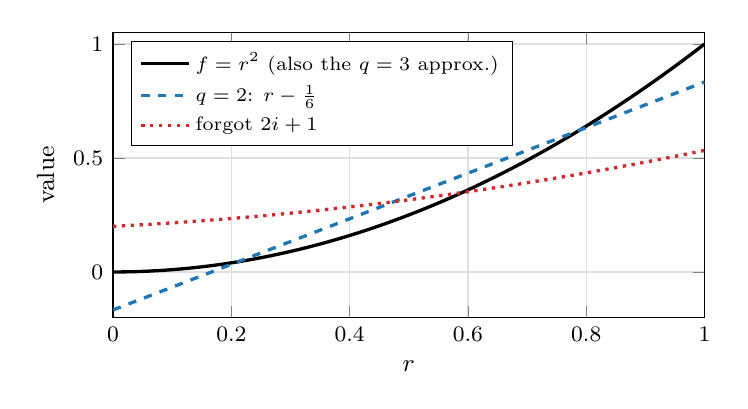
\begin{tikzpicture}
\begin{axis}[width=0.75\textwidth, height=5.2cm, xmin=0, xmax=1, ymin=-0.2, ymax=1.05,
  xlabel={$r$}, ylabel={value}, legend pos=north west, legend cell align=left]
  \addplot[black, very thick, domain=0:1, samples=80] {x^2};
  \addplot[cA, very thick, dashed, domain=0:1, samples=2] {x - 1/6};
  \addplot[cD, very thick, dotted, domain=0:1, samples=80] {0.2 + 2/15*x + 0.2*x^2};
  \legend{$f = r^2$ (also the $q = 3$ approx.), $q = 2$: $r - \frac16$, forgot $2i + 1$}
\end{axis}
\end{tikzpicture}
\end{center}
\begin{result}
$r = \tfrac12\tilde P_0 + \tfrac12\tilde P_1$. \ $r^2 = \tfrac13\tilde P_0 + \tfrac12\tilde P_1 + \tfrac16\tilde P_2$. \ $q = 2$ gives $r - \tfrac16$, with error $\tfrac16\tilde P_2$.
\end{result}

\section{The LMU is a linear dynamical system}

\ans{Q1}
$q = 1$: $\theta A = -1$, $\theta B = 1$, so $A = -2$, $B = 2$ (both $1 \times 1$), $A' = 0.1(-2) + 1 = 0.8$ and $B' = 0.2$. This is $\dot x = (u - x)/\theta$, a \textbf{low-pass filter with time constant $\theta$}.

$q = 2$: $\theta A = \begin{pmatrix} -1 & -1 \\ 3 & -3 \end{pmatrix}$ and $\theta B = \begin{pmatrix} 1 \\ -3 \end{pmatrix}$, so
\[
A = \begin{pmatrix} -2 & -2 \\ 6 & -6 \end{pmatrix}\ (2 \times 2), \quad B = \begin{pmatrix} 2 \\ -6 \end{pmatrix}\ (2 \times 1), \quad
A' = \begin{pmatrix} 0.8 & -0.2 \\ 0.6 & 0.4 \end{pmatrix}, \quad B' = \begin{pmatrix} 0.2 \\ -0.6 \end{pmatrix}.
\]
\begin{lstlisting}[language=Python]
a = nengo.Ensemble(1000, dimensions=q)
nengo.Connection(stim, a, transform=tau * B, synapse=tau)              # B' is q x 1
nengo.Connection(a, a, transform=tau * A + np.eye(q), synapse=tau)     # A' is q x q
\end{lstlisting}

\ans{Q2}
$q = 2$ steady state: $Ax^* + Bu = 0$ gives $-x_1 - x_2 + u = 0$ and $3x_1 - 3x_2 - 3u = 0$, so $x^* = (u, 0)$. A constant window has Legendre coefficients $(u, 0, \dots)$: all of it is on $\tilde P_0$. The stored window is ``$u$ everywhere''.

$q = 1$: the gain of $1/(1 + j\omega\theta)$ is $1/\sqrt{1 + (\omega\theta)^2}$ and the phase is $-\arctan\omega\theta$.
At $1\,\mathrm{Hz}$, $\omega\theta = \pi$, so the amplitude is $1/\sqrt{1 + \pi^2} \approx 0.30$ with a lag of $72^\circ$. At $2\,\mathrm{Hz}$, $\omega\theta = 2\pi$, so the amplitude is $1/\sqrt{1 + 4\pi^2} \approx 0.16$ with a lag of $81^\circ$.

A classifier reads the current value of $x$ only. Both outputs pass through every value in $[-0.16, 0.16]$, so for most of each cycle the instantaneous $x$ is ambiguous. Only near the peaks of the $1\,\mathrm{Hz}$ response ($|x| > 0.16$) does it identify the frequency. Nengo's $q = 1$ classifier has RMSE $0.81$, barely better than outputting $0$.
\begin{center}
\begin{tikzpicture}
\begin{axis}[width=0.9\textwidth, height=5cm, xmin=0, xmax=4, ymin=-1.1, ymax=1.1,
  xlabel={$t$ (s)}, ylabel={value}, legend pos=south west, legend cell align=left, legend columns=2,
  title={$q = 1$ LMU = low-pass with $\theta = 0.5$ s (ideal)}]
  \addplot[gray, thick] table[x=t, y=u] {pn4_data/lmu_q1.dat};
  \addplot[cA, very thick] table[x=t, y=x0] {pn4_data/lmu_q1.dat};
  \legend{$u$, $x_0$}
  \addplot[black, dashed, domain=0:4, samples=2, forget plot] {0.157};
  \addplot[black, dashed, domain=0:4, samples=2, forget plot] {-0.157};
  \node[font=\scriptsize, anchor=south west] at (axis cs:0.05,0.32) {amplitude $0.30$};
  \node[font=\scriptsize, anchor=south west] at (axis cs:2.6,0.17) {$0.16$};
  \draw[black, thin] (axis cs:2,-1.1) -- (axis cs:2,1.1);
\end{axis}
\end{tikzpicture}
\end{center}
\begin{result}
$q = 1$: $A' = 0.8$, $B' = 0.2$, a low-pass with time constant $\theta$. $q = 2$: $A' = \begin{pmatrix} 0.8 & -0.2\\ 0.6 & 0.4\end{pmatrix}$, $B' = \begin{pmatrix} 0.2 \\ -0.6 \end{pmatrix}$. A constant gives $x^* = (u, 0)$. With $q = 1$ the amplitudes are $0.30$ and $0.16$, but most instantaneous values are shared by both frequencies.
\end{result}

\section{Reading the window back out}

\ans{Q1}
With $\tilde P_i(0) = (-1)^i$, $\tilde P_i(1) = 1$ and $\tilde P_i(\tfrac12) = P_i(0)$:
\[
u(t) \approx (1, -1, 1, -1, 1, -1)\,x, \qquad u(t - \theta) \approx (1, 1, 1, 1, 1, 1)\,x, \qquad u(t - \tfrac\theta2) \approx \bigl(1, 0, -\tfrac12, 0, \tfrac38, 0\bigr)\,x.
\]
At the steady state $x = (u, 0, 0, 0, 0, 0)$ all three give $u$: a constant input looks the same at every delay.

\ans{Q2}
\textbf{Average:} $\int_0^1 \tilde P_0 = 1$ and $\int_0^1 \tilde P_i = \langle\tilde P_i, \tilde P_0\rangle = 0$ for $i \ge 1$, so the row is $(1, 0, 0, 0, 0, 0)$: the window mean is $x_0$.

\textbf{Difference:} $u(t) - u(t - \theta) = \sum_i\bigl((-1)^i - 1\bigr)x_i = -2(x_1 + x_3 + x_5)$, with row $(0, -2, 0, -2, 0, -2)$.

\textbf{Energy:} $\int_0^1\bigl(\sum_i x_i\tilde P_i(r)\bigr)^2dr = \sum_{i,j} x_ix_j\langle\tilde P_i, \tilde P_j\rangle = \sum_i \frac{x_i^2}{2i + 1}$, by orthogonality.

The average and the difference are linear in $x$, so each is a \texttt{transform} (a $1 \times q$ matrix) and needs no extra neurons. The energy is quadratic in $x$, so it must be decoded as a \texttt{function} from the $q$-dimensional ensemble.
\begin{result}
Now: $(1, -1, 1, -1, 1, -1)$. \ $\theta$ ago: $(1, \dots, 1)$. \ $\theta/2$ ago: $(1, 0, -\tfrac12, 0, \tfrac38, 0)$. \ Mean: $(1, 0, \dots)$. \ Difference: $-2(x_1 + x_3 + x_5)$. \ Energy $\sum x_i^2/(2i + 1)$ is nonlinear, so it needs neurons.
\end{result}

\section{Classifying the window with \texttt{eval\_points}}

First, the PN4~\S2a plot you should have. The ideal state is drawn thin and the 1000-neuron state thick, for the first three dimensions. The change at $t = 2\,\mathrm{s}$ is clear. The ideal state reaches $\|x\| \approx 1.6$, beyond radius $1$, so the neural state is clipped, most visibly in $x_1$ and $x_2$.
\begin{center}
\begin{tikzpicture}
\begin{axis}[width=0.95\textwidth, height=5.4cm, xmin=0, xmax=4, ymin=-1.6, ymax=1.6,
  xlabel={$t$ (s)}, ylabel={LMU state}, legend style={at={(0.5,1.02)}, anchor=south, legend columns=6},
  legend cell align=left]
  \addplot[cA, very thick] table[x=t, y=x0] {pn4_data/lmu_neural.dat};
  \addplot[cB, very thick] table[x=t, y=x1] {pn4_data/lmu_neural.dat};
  \addplot[cC, very thick] table[x=t, y=x2] {pn4_data/lmu_neural.dat};
  \addplot[cA, thin, forget plot] table[x=t, y=x0] {pn4_data/lmu_ideal.dat};
  \addplot[cB, thin, forget plot] table[x=t, y=x1] {pn4_data/lmu_ideal.dat};
  \addplot[cC, thin, forget plot] table[x=t, y=x2] {pn4_data/lmu_ideal.dat};
  \legend{$x_0$, $x_1$, $x_2$}
  \draw[black, thin] (axis cs:2,-1.6) -- (axis cs:2,1.6);
\end{axis}
\end{tikzpicture}
\end{center}

\ans{Q1}
The output should sit near $+1$ for $t < 2$ and near $-1$ after, with a transition lasting up to $\theta = 0.5\,\mathrm{s}$ after $t = 2$, because the window then holds a mixture of both sines. In Nengo the switch happens within about $0.1\,\mathrm{s}$: the window does not need to be fully refilled before it looks more like $2\,\mathrm{Hz}$. It is also imperfect near $t = 0$, where the window is still filling with the first signal.

Away from the switch it is still not exactly $\pm1$, for three reasons. The 50-neuron category population has its own decoding error and spike noise. The LMU state is noisy and clipped at the radius, so states the decoder saw in training recur only approximately. And the least-squares decoder cannot produce a function that is exactly constant over a whole curved trajectory of states. Over the $1\,\mathrm{Hz}$ part the output is $0.75$--$0.94$; the RMSE over the run is $0.24$.

\ans{Q2}
During training, every start-up state (the state near $0$, with a partly filled window) was labelled $+1$, because training started with $1\,\mathrm{Hz}$. At test time with $2\,\mathrm{Hz}$ first, the start-up states look like those and are labelled $+1$. That lasts until the window holds enough $2\,\mathrm{Hz}$ signal to look different, about the first $0.25\,\mathrm{s}$.

Fixes: (i) do not train on the transients: drop the first $\theta$ of each run from the \texttt{eval\_points} (and ignore the output until the window has filled); (ii) train on both orders, or on many random sequences, so start-up states are not tied to one label; (iii) start the network from a state that reflects past input (for example, run some neutral input first). A shorter $\theta$ also fills faster, but it holds fewer cycles of each frequency.

\begin{center}
\begin{tikzpicture}
\begin{groupplot}[group style={group size=2 by 1, horizontal sep=1.4cm},
  width=0.49\textwidth, height=5cm, xmin=0, xmax=4, ymin=-1.4, ymax=1.4, xlabel={$t$ (s)},
  legend style={at={(0.5,-0.3)}, anchor=north, legend columns=2}, legend cell align=left]
\nextgroupplot[ylabel={category}, title={Trained and tested on $1 \to 2$ Hz}]
  \addplot[black, thick, dashed] coordinates {(0,1) (2,1) (2,-1) (4,-1)};
  \addplot[cA, very thick] table[x=t, y=cat] {pn4_data/lmu_category.dat};
  \legend{target, output}
\nextgroupplot[title={Same decoder, tested on $2 \to 1$ Hz}]
  \addplot[black, thick, dashed] coordinates {(0,-1) (2,-1) (2,1) (4,1)};
  \addplot[cD, very thick] table[x=t, y=catsw] {pn4_data/lmu_category.dat};
  \fill[red!12] (axis cs:0,-1.4) rectangle (axis cs:0.25,1.4);
  \node[font=\scriptsize, anchor=north west, align=left] at (axis cs:0.3,1.35) {start-up says\\``1 Hz''};
  \legend{correct label, output}
\end{groupplot}
\end{tikzpicture}
\end{center}

\textbf{Neuron count.} The RMSE falls with $n$ ($0.52$ at $50$ neurons to $0.18$ at $5000$), quickly at first and then slowly. More neurons represent the 6-D state more accurately, with less distortion in the recurrent loop and less noise. The trend flattens because part of the error does not come from the LMU ensemble: the finite window, the transition after the switch, and the 50-neuron output population.

\textbf{$q$.} The curve is U-shaped: $0.81$ at $q = 1$, $0.51$ at $2$, about $0.24$ at $q = 4$--$8$, then rising to $0.38$ at $32$ and $1.28$ at $64$. Small $q$ cannot hold enough of the window to tell the frequencies apart (Sections~5 and~7). Large $q$ spreads the same $1000$ neurons over more dimensions, so each dimension is represented worse. The high-order coefficients are small and are swamped by noise, and the errors compound through the recurrent loop. At $q = 64$ the network no longer behaves like the LMU at all.
\begin{center}
\begin{tikzpicture}
\begin{groupplot}[group style={group size=2 by 1, horizontal sep=1.5cm},
  width=0.5\textwidth, height=4.8cm, ylabel={classification RMSE}, ymin=0]
\nextgroupplot[xmode=log, xlabel={neurons ($q = 6$)}, title={PN4 \S2d}, ymax=0.6]
  \addplot[cA, very thick, mark=*] table[x=n, y=rmse] {pn4_data/lmu_sweep_n.dat};
\nextgroupplot[xmode=log, log basis x=2, xlabel={$q$ (1000 neurons)}, title={PN4 \S2e}, ymax=1.35]
  \addplot[cD, very thick, mark=*] table[x=q, y=rmse] {pn4_data/lmu_sweep_q.dat};
\end{groupplot}
\end{tikzpicture}
\end{center}
\begin{result}
Expect worst classification for up to $\theta$ after a switch and at start-up. Swapped test: the start-up states were all labelled $+1$; drop transients or train on both orders. RMSE falls and flattens with $n$; it is U-shaped in $q$, best around $4$--$8$.
\end{result}

\section{From least squares to an online rule: the delta rule}

\ans{Q1}
$\partial E/\partial d_j = \bigl(\sum_i d_ia_i - y^{\mathrm d}\bigr)\cdot a_j = \varepsilon a_j$, so $\Delta d_j = -\eta\varepsilon a_j$.
\begin{align*}
\hat y &= 50(0.002) + 100(0.004) = 0.5, \qquad \varepsilon = 0.5 - 0.8 = -0.3,\\
\Delta d &= -10^{-5}(-0.3)(50, 100) = (1.5, 3.0)\times10^{-4}, \qquad d \to (0.00215, 0.0043),\\
\hat y' &= 0.1075 + 0.43 = 0.5375, \qquad \varepsilon' = -0.2625.
\end{align*}
$\|a\|^2 = 2500 + 10000 = 12500$, so $1 - \eta\|a\|^2 = 1 - 0.125 = 0.875$, and $-0.3 \times 0.875 = -0.2625$. \checkmark

\ans{Q2}
$\eta\|a\|^2 = 2.5$, so $\varepsilon_{k+1} = -1.5\,\varepsilon_k$: $\varepsilon = -0.3 \to 0.45 \to -0.675 \to 1.01$, giving $\hat y = 1.25 \to 0.125 \to 1.81$. It overshoots further each step: divergence with alternating sign.

The largest stable rate is $\eta < 2/\|a\|^2 = 1.6\times10^{-4}$. The one-step optimum is $\eta = 1/\|a\|^2 = 8\times10^{-5}$, which zeroes the error in one step.

In a running network $a(x(t))$ changes all the time, so $\|a\|^2$ is not fixed. A rate tuned to zero the error for the current sample over-corrects for this sample and undoes what was learned for other values of $x$ (catastrophic forgetting). A small $\eta$ averages the updates over many samples, which approximates gradient descent on the error over all of them.
\begin{center}
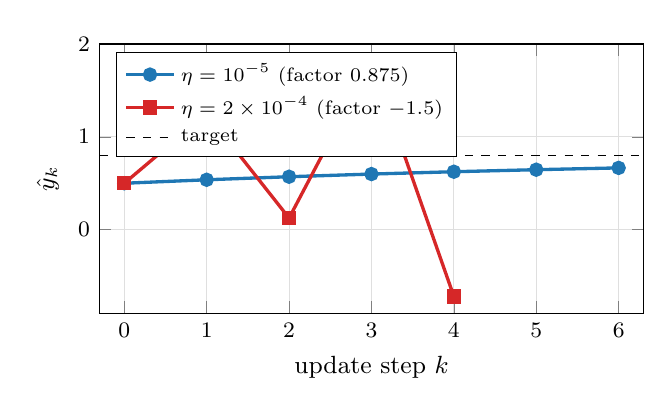
\begin{tikzpicture}
\begin{axis}[width=0.7\textwidth, height=5cm, xmin=-0.3, xmax=6.3, ymin=-0.9, ymax=2.0,
  xlabel={update step $k$}, ylabel={$\hat y_k$}, legend pos=north west, legend cell align=left, xtick={0,...,6}]
  \addplot[cA, very thick, mark=*, samples at={0,...,6}] {0.8 - 0.3*0.875^x};
  \addplot[cD, very thick, mark=square*, samples at={0,...,4}] {0.8 - 0.3*(-1.5)^x};
  \addplot[black, dashed, domain=-0.3:6.3, samples=2] {0.8};
  \legend{$\eta = 10^{-5}$ (factor $0.875$), $\eta = 2\times10^{-4}$ (factor $-1.5$), target}
\end{axis}
\end{tikzpicture}
\end{center}
\begin{result}
$\Delta d = (1.5, 3)\times10^{-4}$; $\hat y: 0.5 \to 0.5375$; $\varepsilon' = 0.875\,\varepsilon$. At $\eta = 2\times10^{-4}$ it diverges. Stable for $\eta < 1.6\times10^{-4}$; one-step optimum $8\times10^{-5}$.
\end{result}

\section{From decoders to synaptic weights: the PES rule}

\ans{Q1}
\[
\Delta w_{1j} = -10^{-4}(2)(+1)(0.25)(80) = -0.004, \qquad \Delta w_{2j} = -10^{-4}(1.5)(-1)(0.25)(80) = +0.003.
\]
The error is positive, so the output is too high. Neuron 1 says ``more positive'' when it fires, so it now receives less drive from the active pre neuron. Neuron 2 says ``more negative'', so it receives more. Both changes lower the decoded output.

\ans{Q2}
With the sign flipped, every update moves the output away from the target: gradient ascent on the error. The error grows, which makes the updates larger. That is positive feedback. The output runs to the edge of the post population's range and stays there, and the weights keep growing. It never learns the identity.

\textbf{Network for $x \mapsto (x^2, -x)$:} \texttt{pre} is 1-D, \texttt{post} is 2-D, \texttt{error} is 2-D.
\begin{center}
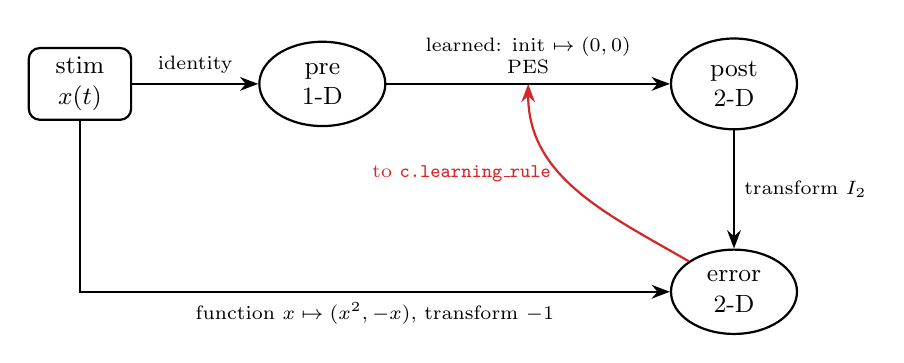
\begin{tikzpicture}[node distance=1.2cm and 2.2cm]
  \node[box] (stim) {stim\\$x(t)$};
  \node[ens, right=1.6cm of stim] (pre) {pre\\1-D};
  \node[ens, right=3.6cm of pre] (post) {post\\2-D};
  \node[ens, below=1.5cm of post] (err) {error\\2-D};
  \draw[-{Stealth}, thick] (stim) -- node[lab, above] {identity} (pre);
  \draw[-{Stealth}, thick] (pre) -- node[lab, above] {learned: init $\mapsto (0, 0)$\\PES} coordinate[midway] (mid) (post);
  \draw[-{Stealth}, thick] (post) -- node[lab, right] {transform $I_2$} (err);
  \draw[-{Stealth}, thick] (stim) |- node[lab, below, pos=0.75] {function $x \mapsto (x^2, -x)$, transform $-1$} (err);
  \draw[-{Stealth}, thick, cD] (err.north west) to[out=150, in=-90] node[lab, left, pos=0.6] {to \texttt{c.learning\_rule}} (mid);
\end{tikzpicture}
\end{center}
\begin{lstlisting}[language=Python]
c = nengo.Connection(pre, post, function=lambda x: [0, 0],
                     learning_rule_type=nengo.PES(learning_rate=1e-4))
nengo.Connection(post, error)
nengo.Connection(stim, error, function=lambda x: [x[0]**2, -x[0]], transform=-1)
nengo.Connection(error, c.learning_rule)
\end{lstlisting}
\begin{result}
$\Delta w_{1j} = -0.004$ and $\Delta w_{2j} = +0.003$; both lower the output. A flipped sign gives positive feedback and divergence. For $(x^2, -x)$: pre 1-D, post and error 2-D, \texttt{initialization} returns $[0, 0]$, and the target enters the error with transform $-1$.
\end{result}

\section{Learning curves: speed, floor, and what you trained on}

\ans{Q1}
Above a floor of about $0.055$ the excess error goes $0.185 \to 0.077 \to 0.028 \to 0.007$, a factor of about $2.5$--$3$ per $2\,\mathrm{s}$, so the time constant is roughly $2\,\mathrm{s}$. The last value is close to the floor: the error that remains after learning, set by representation error, spike noise and weight jitter.

Over $100\,\mathrm{s}$ at $\eta = 10^{-4}$, the first $10\,\mathrm{s}$ repeat this curve. After that it fluctuates around $0.04$ ($0.03$--$0.07$), and the bumps come when the white-noise input wanders into values it has rarely visited. With $\eta = 10^{-5}$ it is about ten times slower: still about $0.2$ at $10\,\mathrm{s}$, and down to the same floor only after about $60\,\mathrm{s}$. Over $100\,\mathrm{s}$ it ends about where the fast rate does ($0.047$ against $0.039$ over the last $20\,\mathrm{s}$). The floor is set mainly by the populations, not by $\eta$.
\begin{center}
\begin{tikzpicture}
\begin{groupplot}[group style={group size=2 by 1, horizontal sep=1.5cm},
  width=0.48\textwidth, height=5cm, ymin=0, legend cell align=left]
\nextgroupplot[xlabel={$t$ (s)}, ylabel={value}, xmin=0, xmax=10, ymin=-0.95, ymax=0.95,
  title={PN4 \S3a: learning the identity}, legend pos=south east, legend columns=2]
  \addplot[gray, thick] table[x=t, y=u] {pn4_data/pes_identity.dat};
  \addplot[cA, thick] table[x=t, y=out] {pn4_data/pes_identity.dat};
  \legend{input, output}
\nextgroupplot[xlabel={$t$ (s), chunk centre}, ylabel={RMSE per 2-s chunk}, xmin=0, xmax=100, ymax=0.32,
  title={PN4 \S3c--e}, legend pos=north east]
  \addplot[cA, thick, mark=*, mark size=1pt] table[x=tmid, y=rmse] {pn4_data/pes_rmse100_1e4.dat};
  \addplot[cD, thick, mark=*, mark size=1pt] table[x=tmid, y=rmse] {pn4_data/pes_rmse100_1e5.dat};
  \addplot[black, only marks, mark=square*, mark size=1.8pt] table[x=tmid, y=rmse] {pn4_data/pes_rmse10.dat};
  \legend{$\eta = 10^{-4}$ ($100$ s), $\eta = 10^{-5}$ ($100$ s), {$\eta = 10^{-4}$ ($10$ s, $10$ runs)}}
\end{groupplot}
\end{tikzpicture}
\end{center}

\ans{Q2}
With \texttt{rms=0.3}, $|x| > 0.6$ is a two-standard-deviation event and $|x| > 0.9$ almost never happens. PES only changes the weights in response to the activity of the inputs it is shown, so the learned function is good near the middle and poor near the ends. On a ramp from $-1$ to $1$ the error is largest at both ends.

Changes that make the learned function more accurate:
\begin{enumerate}[label=(\roman*), leftmargin=1.8em, itemsep=1pt, topsep=2pt]
\item Train on inputs that cover the whole range (larger \texttt{rms}, or ramps). This targets the gaps in what was trained.
\item More neurons in \texttt{pre} and \texttt{post}. This targets representation error and spike noise.
\item More neurons in \texttt{error}, or a filtered error. This targets noise in the teaching signal.
\item Train longer and then lower $\eta$, or let $\eta$ decay over time. This targets weight jitter while keeping the early speed.
\end{enumerate}
\begin{result}
Time constant about $2\,\mathrm s$ at $\eta = 10^{-4}$, floor about $0.04$--$0.06$. $\eta = 10^{-5}$ is about ten times slower to the same floor. Accuracy is worst where training rarely went; cover the range, add neurons, lower the noise, and decay $\eta$.
\end{result}

\section{Adaptive control: learning the force you did not model}

\ans{Q1}
At rest, $\ddot\theta = \dot\theta = 0$, so $k_p(0 - \theta) = mgL\cos\theta$, that is $-25\theta = 9.8\cos\theta$. With $\cos\theta \approx 1$, $\theta \approx -9.8/25 = -0.39\,\mathrm{rad}$. The magnitude is too large, because $\cos\theta < 1$ once $\theta \ne 0$, so gravity is weaker than assumed. The exact root is $\theta = -0.366\,\mathrm{rad}$ (about $21^\circ$ below horizontal).

Linearized: $\ddot\theta + k_d\dot\theta + k_p\theta = -g$, with characteristic roots $s^2 + 10s + 25 = (s + 5)^2$. This is critically damped: no oscillation, time constant $0.2\,\mathrm{s}$. From $\pi/4$ the arm swings down past $0$ and settles at $-0.366$ within about $1$--$1.5\,\mathrm{s}$.

\ans{Q2}
\begin{center}
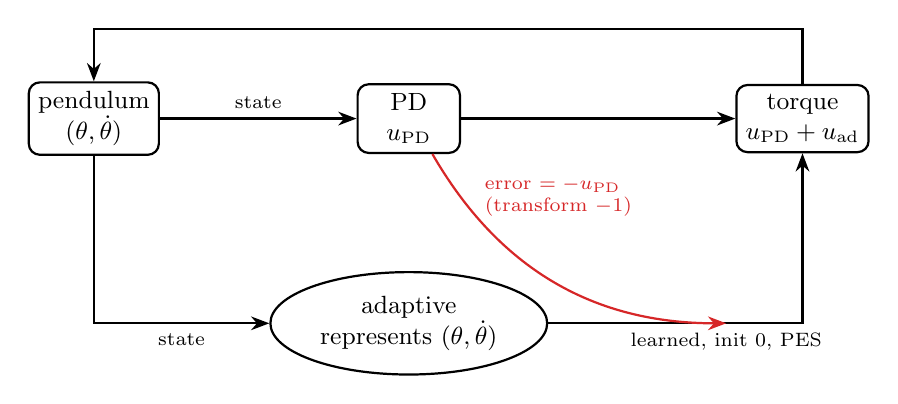
\begin{tikzpicture}
  \node[box] (plant) at (0,0) {pendulum\\$(\theta, \dot\theta)$};
  \node[box] (pd) at (4,0) {PD\\$u_{\mathrm{PD}}$};
  \node[box] (tq) at (9,0) {torque\\$u_{\mathrm{PD}} + u_{\mathrm{ad}}$};
  \node[ens] (ad) at (4,-2.6) {adaptive\\represents $(\theta, \dot\theta)$};
  \draw[-{Stealth}, thick] (plant) -- node[lab, above] {state} (pd);
  \draw[-{Stealth}, thick] (pd) -- (tq);
  \draw[-{Stealth}, thick] (plant) |- node[lab, below, pos=0.75] {state} (ad);
  \draw[-{Stealth}, thick] (ad.east) -| coordinate[pos=0.35] (lm) (tq.south);
  \node[lab, below] at (lm) {learned, init $0$, PES};
  \draw[-{Stealth}, thick, cD] (pd.south) ++(0.3,0) to[out=-60, in=180] (lm);
  \node[lab, text=cD, align=left] at (5.9,-1.0) {error $= -u_{\mathrm{PD}}$\\(transform $-1$)};
  \draw[-{Stealth}, thick] (tq.north) |- ++(0,0.7) -| (plant.north);
\end{tikzpicture}
\end{center}
The error is $\varepsilon = -u_{\mathrm{PD}}$, so the connection into \texttt{conn.learning\_rule} has \texttt{transform=-1}. If the PD controller is still pushing up ($u_{\mathrm{PD}} > 0$), the adaptive output must increase, and PES increases the output when $\varepsilon < 0$. At $\theta^* = 0$ the arm can only rest at $\theta = 0$ with $u_{\mathrm{PD}} = 0$ when $u_{\mathrm{ad}} = mgL\cos 0 = 9.8$. Nengo learns $9.80$.

PD-only at $\theta^* = 0.8$: solve $25(0.8 - \theta) = 9.8\cos\theta$. At $\theta = 0.446$, the left side is $25 \times 0.354 = 8.85$ and the right side is $9.8 \times 0.902 = 8.84$. \checkmark

A constant learned torque of $9.8$: solve $25(0.8 - \theta) + 9.8 = 9.8\cos\theta$, which gives $\theta \approx 0.97$. The arm overshoots the target by about $0.17\,\mathrm{rad}$, because at $0.8$ gravity needs only $9.8\cos0.8 = 6.83$. The required torque depends on $\theta$, so the adaptive population must represent $\theta$ to output $mgL\cos\theta$, the right amount at every angle. In Nengo, after four cycles the error at $\theta^* = 0$ has fallen from $-0.19$ to $-0.03$, and at $0.8$ it is about $+0.02$, while PD-only stays at $-0.37$ and $-0.35$.
\begin{center}
\begin{tikzpicture}
\begin{groupplot}[group style={group size=1 by 2, vertical sep=1.4cm},
  width=0.95\textwidth, height=4.6cm, xmin=0, xmax=40, legend cell align=left]
\nextgroupplot[ylabel={$\theta$ (rad)}, ymin=-0.55, ymax=1.05, legend style={at={(0.5,1.03)}, anchor=south, legend columns=3},
  title={}]
  \addplot[black, thick, dashed] table[x=t, y=target] {pn4_data/pendulum.dat};
  \addplot[cD, very thick] table[x=t, y=thpd] {pn4_data/pendulum.dat};
  \addplot[cA, very thick] table[x=t, y=thad] {pn4_data/pendulum.dat};
  \legend{target $\theta^*$, PD only, PD + adaptive (PES)}
\nextgroupplot[xlabel={$t$ (s)}, ylabel={$u_{\mathrm{ad}}$ (N\,m)}, ymin=-2, ymax=12, legend pos=south east]
  \addplot[cA, very thick] table[x=t, y=uad] {pn4_data/pendulum.dat};
  \addplot[black, dashed, domain=0:40, samples=2] {9.8};
  \addplot[gray, dashed, domain=0:40, samples=2] {6.83};
  \legend{learned torque, $mgL\cos 0 = 9.8$, $mgL\cos 0.8 = 6.83$}
\end{groupplot}
\end{tikzpicture}
\end{center}
\begin{result}
PD-only steady angle $-0.366$ (estimate $-0.39$), critically damped. Error into the learning rule $= -u_{\mathrm{PD}}$, and the population learns $u_{\mathrm{ad}} \approx mgL\cos\theta$. PD-only at $0.8$ settles at $0.446$; a constant $9.8$ overshoots to $0.97$. The state must be represented because the needed torque depends on $\theta$.
\end{result}

\section{What the SVD of $\gamma$ says, computed by hand}

\ans{Q1}
\[
\mathbf A = \begin{pmatrix} 0 & 2 \\ 1 & 1 \\ 2 & 0 \end{pmatrix}, \qquad
\gamma = \mathbf A^\T\mathbf A = \begin{pmatrix} 5 & 1 \\ 1 & 5 \end{pmatrix}, \qquad
S = (6, 4), \qquad \mathbf U = \tfrac{1}{\sqrt2}\begin{pmatrix} 1 & 1 \\ 1 & -1 \end{pmatrix}.
\]
$\chi_1 = \mathbf A u_1 = \tfrac1{\sqrt2}(2, 2, 2) = \sqrt2\,(1, 1, 1)$, a \textbf{constant}. $\chi_2 = \mathbf A u_2 = \tfrac{1}{\sqrt2}(-2, 0, 2) = \sqrt2\,(-1, 0, 1)$, \textbf{linear} in $x$. Check: $\|\chi_1\|^2 = 6 = S_1$ and $\|\chi_2\|^2 = 4 = S_2$.

Decoder for $x$: $\mathbf A^\T\mathbf X = (2, -2)$, and $\gamma^{-1} = \frac{1}{24}\begin{pmatrix} 5 & -1 \\ -1 & 5\end{pmatrix}$, so $\mathbf D = \frac{1}{24}(12, -12) = (\tfrac12, -\tfrac12)$. Check: $\tfrac12(1 + x) - \tfrac12(1 - x) = x$. \checkmark

$x^2$ at the samples is $(1, 0, 1)$. With two neurons the population spans only two functions, $\mathrm{span}\{1, x\}$. The best attempt is the projection onto that span: $(1, 0, 1) = \tfrac23(1, 1, 1) + \tfrac13(1, -2, 1)$, so $\hat f = \tfrac23$ everywhere, and the part $\tfrac13(1, -2, 1)$ cannot be decoded.

\ans{Q2}
$\langle\chi_2, x\rangle = \sqrt2\cdot2 = 2\sqrt2$, so $\Phi_2 = 2\sqrt2/(4 + 4) = \sqrt2/4$ and $\hat x = \chi_2\Phi_2 = \tfrac12(-1, 0, 1) = \tfrac12 x$.

$\langle\chi_1, 1\rangle = 3\sqrt2$, so $\Phi_1 = 3\sqrt2/(6 + 4)$ and $\hat 1 = \tfrac{6}{10} = 0.6$ at every point.

In general, the component on $\chi_m$ is scaled by $S_m/(S_m + \sigma^2)$: $4/8 = 0.5$ for $x$ and $6/10 = 0.6$ for the constant. The linear function is shrunk more because its singular value is smaller, so the same noise is a larger fraction of it.

Doubling both rates multiplies $\mathbf A$ by $2$ and $\gamma$ by $4$, so $S = (24, 16)$, with the same $\mathbf U$. Now $\hat x = \frac{16}{20}x = 0.8x$. The noise did not grow, so higher rates mean a higher signal-to-noise ratio in every direction.
\begin{result}
$\gamma = \begin{pmatrix} 5 & 1 \\ 1 & 5\end{pmatrix}$, $S = (6, 4)$, $\chi_1 \propto 1$, $\chi_2 \propto x$, $\mathbf D = (\tfrac12, -\tfrac12)$. Two neurons cannot decode $x^2$ (best is $\tfrac23$). With $\sigma^2 = 4$: $\hat x = 0.5x$, $\hat 1 = 0.6$. Doubling the rates gives $S = (24, 16)$ and $\hat x = 0.8x$.
\end{result}

\section{The spectrum of a real population}

\ans{Q1}
About $8$ singular values are clearly above the noise level, and the $9$th sits on it. Beyond that, the directions are mostly noise.

Expected shapes (Nengo, normalized, with the Legendre polynomials $P_1$--$P_4$ dashed): $\chi_1$ is a near-constant (the mean firing, rising a little with $x$), $\chi_2$ is linear, $\chi_3$ quadratic, $\chi_4$ cubic, and $\chi_5$ quartic.
\begin{center}
\begin{tikzpicture}
\begin{axis}[width=0.9\textwidth, height=5.4cm, xmin=-1, xmax=1, ymin=-1.1, ymax=1.1,
  xlabel={$x$}, ylabel={$\chi_m(x)$ (scaled)}, legend style={at={(0.5,1.03)}, anchor=south, legend columns=5}, legend cell align=left]
  \addplot[black, very thick] table[x=x, y=c0] {pn4_data/svd_chi.dat};
  \addplot[cA, very thick] table[x=x, y=c1] {pn4_data/svd_chi.dat};
  \addplot[cB, very thick] table[x=x, y=c2] {pn4_data/svd_chi.dat};
  \addplot[cC, very thick] table[x=x, y=c3] {pn4_data/svd_chi.dat};
  \addplot[cE, very thick] table[x=x, y=c4] {pn4_data/svd_chi.dat};
  \legend{$\chi_1$, $\chi_2$, $\chi_3$, $\chi_4$, $\chi_5$}
  \addplot[cA, dashed, domain=-1:1, samples=2, forget plot] {x};
  \addplot[cB, dashed, domain=-1:1, samples=60, forget plot] {(3*x^2-1)/2};
  \addplot[cC, dashed, domain=-1:1, samples=60, forget plot] {(5*x^3-3*x)/2};
  \addplot[cE, dashed, domain=-1:1, samples=80, forget plot] {(35*x^4-30*x^2+3)/8};
\end{axis}
\end{tikzpicture}
\end{center}
Easiest to hardest:
\begin{enumerate}[label=(\arabic*), leftmargin=1.8em, itemsep=1pt, topsep=2pt]
\item $x$: almost entirely $\chi_2$ ($S_2/S_1 \approx 0.5$).
\item $x^2$: needs $\chi_1$ and $\chi_3$ ($S_3/S_1 \approx 0.07$), still well above the noise.
\item $|x|$: even and smooth, but the kink at $0$ needs many even-order terms whose singular values reach the noise level.
\item $\mathrm{sign}(x)$: discontinuous, so it needs odd terms of every order. Most of them are below the noise, so the decoded version is a smoothed ramp with ripples.
\end{enumerate}
This is exactly the \texttt{choice} plot in Section~4. Its jumps live on high-order basis functions that are not available, so the decoder gives the low-order approximation: rounded corners and wiggles.

\ans{Q2}
$N_S(l, 2) = l + 1$, so the orders $l = 0, 1, 2, 3, 4$ have $1, 2, 3, 4, 5$ singular values, in plateaus that step down with order. The Nengo spectrum (300 neurons, 2-D) shows exactly these groups. In 4-D, $N_S(2, 4) = \frac{5!}{2!\,3!} = 10$ second-order terms.

$x_1x_2$ is a second-order term, like $x_1^2$ and $x_2^2$, and all terms of one order have singular values of about the same size. So it is about as easy to decode as $x_1^2$, provided the population represents both variables together.

Clumped intercepts break the ordering. If all ``on'' neurons switch on near $x_{\max}$ and all ``off'' neurons near $x_{\min}$, the population mostly varies near the ends of the range. Its activity is not dominated by a linear trend, so the linear term is not better supported than the quadratic one. The tidy Legendre ordering depends on heterogeneous tuning curves that tile the range.
\begin{center}
\begin{tikzpicture}
\begin{semilogyaxis}[width=0.8\textwidth, height=5cm, xmin=0, xmax=21.5, ymin=3e-4, ymax=2,
  xlabel={index $m$}, ylabel={$S_m/S_1$}, title={2-D population: plateaus of $1, 2, 3, 4, 5$ values}, xtick={1,2,4,7,11,16,21}]
  \addplot[cA, only marks, mark=*, mark size=1.8pt] table[x=m, y=s] {pn4_data/svd_spectrum_2d.dat};
  \node[font=\scriptsize] at (axis cs:1,0.45) {$l{=}0$};
  \node[font=\scriptsize] at (axis cs:2.5,0.09) {$l{=}1$};
  \node[font=\scriptsize] at (axis cs:5,0.009) {$l{=}2$};
  \node[font=\scriptsize] at (axis cs:8.5,0.0019) {$l{=}3$};
  \node[font=\scriptsize] at (axis cs:13,0.0008) {$l{=}4$};
\end{semilogyaxis}
\end{tikzpicture}
\end{center}
\begin{result}
About $8$ usable basis functions, Legendre-like. Order of difficulty: $x$, $x^2$, $|x|$, $\mathrm{sign}(x)$. In 2-D the orders have $1, 2, 3, 4, 5$ values; in 4-D there are $10$ second-order terms; $x_1x_2$ is about as hard as $x_1^2$. Clumping breaks the ordering.
\end{result}

\section{Unsupervised learning: PCA, Hebb, Oja, and STDP}

\ans{Q1}
$\sum x_1^2 = 4 + 4 + 1 + 1 = 10$, $\sum x_2^2 = 10$, $\sum x_1x_2 = 2 + 2 + 2 + 2 = 8$. So
\[
C = \frac13\begin{pmatrix} 10 & 8 \\ 8 & 10 \end{pmatrix}, \qquad \lambda_1 = \tfrac{18}{3} = 6 \ \text{along}\ \tfrac{1}{\sqrt2}(1, 1), \qquad \lambda_2 = \tfrac23 \ \text{along}\ \tfrac{1}{\sqrt2}(1, -1).
\]
The first component carries $6/(6 + \tfrac23) = 0.9$ of the variance. Oja's rule takes the weight vector to $\pm\frac{1}{\sqrt2}(1, 1)$, unit length, along the first principal component. The sign depends on the starting weights.

\ans{Q2}
\textbf{Hebb.} With $a_i = w_i^\T a$: $\Delta w_i = \eta a_ia = \eta\,a a^\T w_i$, so $\mathbb{E}[\Delta w_i] = \eta Cw_i$ for centred inputs. This is $\dot w = \eta Cw$, a linear system whose eigenvalues are $\eta\lambda_k > 0$. Every component grows exponentially, fastest along the first principal component, and nothing stops it.

\textbf{Oja.} In vector form $\Delta w_i = \eta(a_ia - a_i^2 w_i)$, so $\mathbb{E}[\Delta w_i] = \eta\bigl(Cw_i - (w_i^\T Cw_i)w_i\bigr)$. At a fixed point $Cw_i = (w_i^\T Cw_i)w_i$, so $w_i$ is an eigenvector of $C$, $Cw_i = \lambda w_i$. Substituting back gives $\lambda = \lambda\|w_i\|^2$, so $\|w_i\| = 1$. Only the top eigenvector is a stable fixed point.

\textbf{STDP.} Pre at $10$, post at $15$: $\Delta t = +5\,\mathrm{ms}$, so $W = \alpha^+e^{-0.5} \approx 0.61\alpha^+$, potentiation. Pre at $10$, post at $5$: $\Delta t = -5\,\mathrm{ms}$, so $W = -\alpha^-e^{-0.5} \approx -0.61\alpha^-$, depression. The pre spike came after the post spike, so it cannot have caused it.
\begin{center}
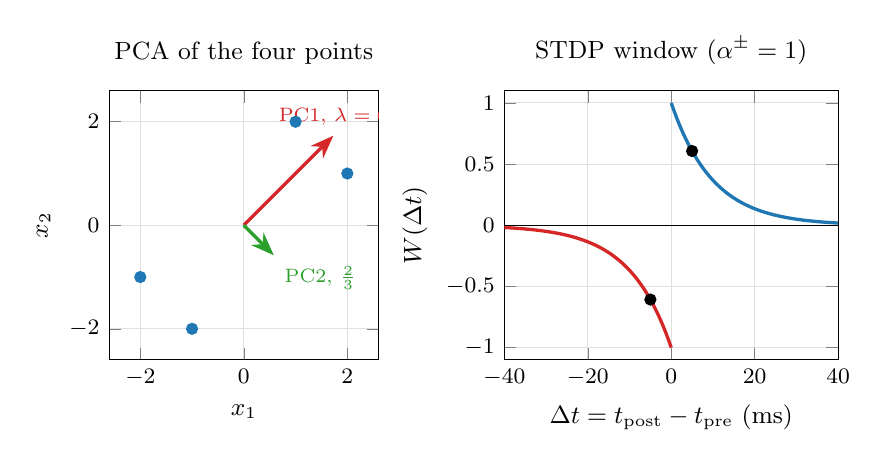
\begin{tikzpicture}
\begin{groupplot}[group style={group size=2 by 1, horizontal sep=1.6cm}, width=0.48\textwidth, height=5cm]
\nextgroupplot[axis equal image, xmin=-2.6, xmax=2.6, ymin=-2.6, ymax=2.6, xlabel={$x_1$}, ylabel={$x_2$}, title={PCA of the four points}]
  \addplot[only marks, mark=*, cA] coordinates {(2,1) (-2,-1) (1,2) (-1,-2)};
  \draw[-{Stealth}, very thick, cD] (axis cs:0,0) -- (axis cs:1.73,1.73) node[above, font=\scriptsize] {PC1, $\lambda = 6$};
  \draw[-{Stealth}, very thick, cC] (axis cs:0,0) -- (axis cs:0.58,-0.58) node[below right, font=\scriptsize] {PC2, $\frac23$};
\nextgroupplot[xmin=-40, xmax=40, ymin=-1.1, ymax=1.1, xlabel={$\Delta t = t_{\mathrm{post}} - t_{\mathrm{pre}}$ (ms)}, ylabel={$W(\Delta t)$}, title={STDP window ($\alpha^\pm = 1$)}]
  \addplot[cA, very thick, domain=0.01:40, samples=80] {exp(-x/10)};
  \addplot[cD, very thick, domain=-40:0, samples=80] {-exp(x/10)};
  \addplot[only marks, mark=*, black] coordinates {(5,0.607) (-5,-0.607)};
  \addplot[black, domain=-40:40, samples=2] {0};
\end{groupplot}
\end{tikzpicture}
\end{center}
\begin{result}
$C = \frac13\begin{pmatrix}10 & 8\\8 & 10\end{pmatrix}$, eigenvalues $6$ and $\tfrac23$, PC1 $= \tfrac{1}{\sqrt2}(1, 1)$ with $90\%$ of the variance; Oja converges there. Hebb gives $\dot w = \eta Cw$, which diverges. STDP: $+0.61\alpha^+$ (pre before post) and $-0.61\alpha^-$ (pre after post).
\end{result}

%=====================================================================
\part*{Part C}
%=====================================================================

\ans{Q1}
The decoder learning rule, averaged over the inputs, is $\dot d = -\eta\sum_k a(x_k)\bigl(a(x_k)^\T d - f_k\bigr) = -\eta(\gamma d - \mathbf A^\T f)$. Rotate into the SVD basis with $\Phi = \mathbf U^\T d$ and $\gamma = \mathbf U\mathbf S\mathbf U^\T$:
\[
\dot\Phi_m = -\eta\bigl(S_m\Phi_m - \langle\chi_m, f\rangle\bigr) = -\eta S_m\bigl(\Phi_m - \Phi_m^*\bigr), \qquad \Phi_m^* = \frac{\langle\chi_m, f\rangle}{S_m}.
\]
Each coefficient relaxes independently with time constant $1/(\eta S_m)$. The linear part of a function lives on $\chi_2$ ($S_2/S_1 \approx 0.52$). The quadratic part of $x^2$ lives on $\chi_3$ ($S_3/S_1 \approx 0.068$), so it is learned about $0.52/0.068 \approx 8$ times more slowly than the linear part, and about $15$ times more slowly than the constant part on $\chi_1$. The same small singular value that makes $x^2$ harder to decode makes it slower to learn. In Nengo ($\eta = 10^{-4}$, input \texttt{rms=0.5}), the relative error for $x^2$ falls more slowly and levels off at about twice that for $x$:
\begin{center}
\begin{tikzpicture}
\begin{axis}[width=0.75\textwidth, height=4.8cm, xmin=0, xmax=60, ymin=0, ymax=0.95,
  xlabel={$t$ (s), chunk centre}, ylabel={RMSE / s.d.\ of target}, legend pos=north east, legend cell align=left]
  \addplot[cA, very thick, mark=*, mark size=1pt] table[x=tmid, y=relrmse] {pn4_data/pes_rel_lin.dat};
  \addplot[cD, very thick, mark=*, mark size=1pt] table[x=tmid, y=relrmse] {pn4_data/pes_rel_sq.dat};
  \legend{learning $f = x$, learning $f = x^2$}
\end{axis}
\end{tikzpicture}
\end{center}

\ans{Q2}
Accumulator: the noisy ramps cross $0.9$ at $0.44\,\mathrm{s}$ ($u = 0.2$) and $1.05\,\mathrm{s}$ ($u = -0.1$). Both are later than without noise ($0.36$ and $0.82$), because the noise makes the loop slightly leaky (Section~3). The decision output stays near $0$ and then ramps to about $\pm1$ as the accumulator passes $0.9$. With default intercepts it wiggles by up to $0.17$--$0.34$ beforehand; with \texttt{Uniform(0.4, 0.9)} it is exactly $0$ until the decision.

The model does decide faster with stronger evidence: about $0.44\,\mathrm{s}$ against $1.1\,\mathrm{s}$ for half the evidence, roughly $2.5\times$ slower. The weak case is less clean. Its accumulator hovers near $-0.95$, on the steep part of the decoded \texttt{choice}, so the output only reaches about $-0.6$ and flickers. With the high intercepts it crosses $-0.5$ later ($1.34\,\mathrm{s}$), because the population has to be driven past $0.4$ before it fires at all.
\begin{center}
\begin{tikzpicture}
\begin{groupplot}[group style={group size=2 by 1, horizontal sep=1.4cm},
  width=0.49\textwidth, height=5.2cm, xmin=0, xmax=2, ymin=-1.3, ymax=1.3, xlabel={$t$ (s)},
  legend style={at={(1.1,-0.3)}, anchor=north, legend columns=4}, legend cell align=left]
\nextgroupplot[ylabel={value}, title={default decision intercepts}]
  \addplot[cA, thin] table[x=t, y=acc02] {pn4_data/decision_default.dat};
  \addplot[cA, very thick] table[x=t, y=out02] {pn4_data/decision_default.dat};
  \addplot[cD, thin] table[x=t, y=accm01] {pn4_data/decision_default.dat};
  \addplot[cD, very thick] table[x=t, y=outm01] {pn4_data/decision_default.dat};
  \addplot[gray, dotted, thick, domain=0:2, samples=2, forget plot] {0.9};
  \addplot[gray, dotted, thick, domain=0:2, samples=2, forget plot] {-0.9};
  \legend{accumulator $u{=}0.2$, decision $u{=}0.2$, accumulator $u{=}{-0.1}$, decision $u{=}{-0.1}$}
\nextgroupplot[title={\texttt{intercepts=Uniform(0.4, 0.9)}}]
  \addplot[cA, thin] table[x=t, y=acc02] {pn4_data/decision_highint.dat};
  \addplot[cA, very thick] table[x=t, y=out02] {pn4_data/decision_highint.dat};
  \addplot[cD, thin] table[x=t, y=accm01] {pn4_data/decision_highint.dat};
  \addplot[cD, very thick] table[x=t, y=outm01] {pn4_data/decision_highint.dat};
  \addplot[gray, dotted, thick, domain=0:2, samples=2, forget plot] {0.9};
  \addplot[gray, dotted, thick, domain=0:2, samples=2, forget plot] {-0.9};
\end{groupplot}
\end{tikzpicture}
\end{center}

\ans{Q3}
\begin{center}
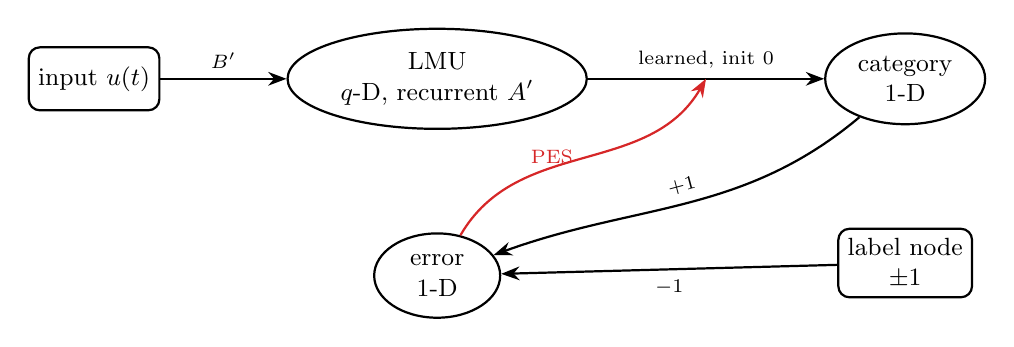
\begin{tikzpicture}[node distance=1.2cm and 2cm]
  \node[box] (u) {input $u(t)$};
  \node[ens, right=1.6cm of u] (lmu) {LMU\\$q$-D, recurrent $A'$};
  \node[ens, right=3cm of lmu] (cat) {category\\1-D};
  \node[box, below=1.3cm of cat] (lab) {label node\\$\pm1$};
  \node[ens, below=1.3cm of lmu] (err) {error\\1-D};
  \draw[-{Stealth}, thick] (u) -- node[lab, above] {$B'$} (lmu);
  \draw[-{Stealth}, thick] (lmu) -- node[lab, above] {learned, init $0$} coordinate[midway] (m) (cat);
  \draw[-{Stealth}, thick] (cat) to[out=-140, in=20] node[lab, above, sloped] {$+1$} (err);
  \draw[-{Stealth}, thick] (lab) -- node[lab, below] {$-1$} (err);
  \draw[-{Stealth}, thick, cD] (err) to[out=60, in=-120] node[lab, left] {PES} (m);
\end{tikzpicture}
\end{center}
The error computes output $-$ label, using a node that supplies the correct label during training. Advantage: it learns online from the states the spiking network actually produces, including spike noise and the clipping at the radius, and it can keep adapting if the signals change. Disadvantages: it needs the label at run time, it takes many seconds to converge, and it suffers from catastrophic forgetting. Two seconds of $1\,\mathrm{Hz}$ followed by two seconds of $2\,\mathrm{Hz}$ lets the second block overwrite the first, so the two must be interleaved many times.

\ans{Q4}
(a) $\gamma = \mathbf A^\T\mathbf A$ is built only from the tuning curves; the target function appears only in $\mathbf A^\T\mathbf X$. So its singular values describe what the population can decode, before you choose what to decode.
(b) Pre-computed decoders are fitted to the static rate curves $G[J]$, not to the filtered spike trains and synaptic dynamics the network actually has. PES adjusts the weights using the real spiking activity and the real error, so it can correct for those mismatches, and it can end with a lower error than the offline solution.
(c) The target is the torque that would make the arm follow the reference exactly, which depends on the unmodelled gravity. We never need to know it. The PD output already tells us the direction and size of the remaining correction, and it is zero only when the target torque has been reached.

%=====================================================================
\part*{Part D \quad Practice Test 4 solutions}
%=====================================================================

\ans{1(a)} [1] $A' = 1 \Rightarrow A = 0$. $B = B'/\tau = 0.5/0.05 = 10\,\mathrm{s^{-1}}$. So $\dot x = 10u$.

\ans{1(b)} [2] Slope $10 \times 0.2 = 2\,\mathrm{s^{-1}}$, so $x = 0.8$ at $0.4\,\mathrm{s}$ (1 mark). Offset $(1 - 0.005/0.05) \times 0.5 \times 0.2 = 0.9 \times 0.1 = 0.09$, so $0.8$ is reached at $(0.8 - 0.09)/2 = 0.355\,\mathrm{s}$ (1 mark).

\ans{1(c)} [1] $u = 0.2$: jump to $0.09$, slope $2$, flattening just above $1$ at about $0.46\,\mathrm{s}$. $u = -0.1$: jump to $-0.045$, slope $-1$, flattening just below $-1$ at about $0.96\,\mathrm{s}$. Marks for the offset, the slopes, and stopping just past $\pm1$ rather than at exactly $\pm1$.
\begin{center}
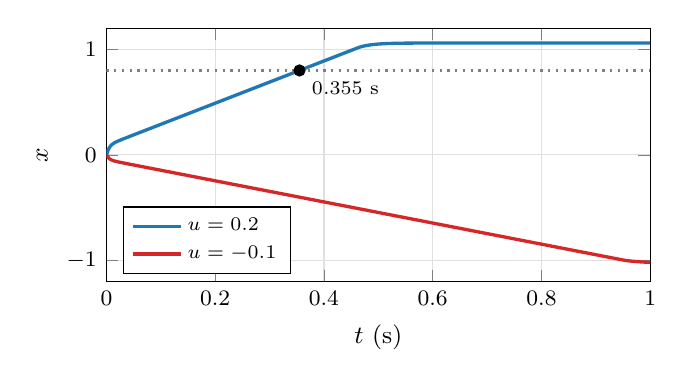
\begin{tikzpicture}
\begin{axis}[width=0.7\textwidth, height=4.8cm, xmin=0, xmax=1, ymin=-1.2, ymax=1.2,
  xlabel={$t$ (s)}, ylabel={$x$}, legend pos=south west, legend cell align=left]
  \addplot[cA, very thick, domain=0:1, samples=300] {min(2*x + 0.09*(1-exp(-x/0.005)), 1 + 0.06*(1-exp(-max(2*x+0.09-1,0)/0.05)))};
  \addplot[cD, very thick, domain=0:1, samples=300] {max(-x - 0.045*(1-exp(-x/0.005)), -1 - 0.03*(1-exp(-max(x+0.045-1,0)/0.05)))};
  \legend{$u = 0.2$, $u = -0.1$}
  \addplot[gray, dotted, thick, domain=0:1, samples=2, forget plot] {0.8};
  \addplot[only marks, mark=*, black, forget plot] coordinates {(0.355,0.8)};
  \node[font=\scriptsize, anchor=north west] at (axis cs:0.36,0.78) {$0.355$ s};
\end{axis}
\end{tikzpicture}
\end{center}

\ans{2(a)} [2]
\[
A = \begin{pmatrix} -1 & -1 & -1 \\ 3 & -3 & -3 \\ -5 & 5 & -5 \end{pmatrix},\quad B = \begin{pmatrix} 1 \\ -3 \\ 5 \end{pmatrix},\quad
A' = \begin{pmatrix} 0.9 & -0.1 & -0.1 \\ 0.3 & 0.7 & -0.3 \\ -0.5 & 0.5 & 0.5 \end{pmatrix},\quad B' = \begin{pmatrix} 0.1 \\ -0.3 \\ 0.5 \end{pmatrix}.
\]
\ans{2(b)} [2] $u(t - \theta)$: $(1, 1, 1)$. $u(t - \theta/2)$: $(1, 0, -\tfrac12)$. Window average: $(1, 0, 0)$. For a constant input, $Ax^* + Bu = 0$ gives $x^* = (u, 0, 0)$ (check: row 1 gives $-u + u = 0$, row 2 gives $3u - 3u = 0$, row 3 gives $-5u + 5u = 0$). Every row then gives $u$.

\ans{2(c)} [1] A delay is a linear function of the window, so it is a fixed linear combination of the Legendre coefficients: a \texttt{transform}. ``Which frequency'' is a nonlinear function of the window (it does not scale or add linearly with $u$), so it must be decoded from neurons as a \texttt{function}.

\ans{3(a)} [2] $\hat y = 0.3 + 0.2 = 0.5$, so $\varepsilon = 0.5 - 0.1 = 0.4$. $\Delta d = -10^{-4}(0.4)(30, 40) = (-0.0012, -0.0016)$. $\|a\|^2 = 2500$ and $\eta\|a\|^2 = 0.25$, so $\varepsilon' = 0.4 \times 0.75 = 0.3$ ($\hat y = 0.4$). Stable, since $0 < 0.25 < 2$.

\ans{3(b)} [1] $\Delta w_{ij} = -\eta\,\alpha_i\langle e_i, \varepsilon\rangle\,a_j$. The post neuron's own $\alpha_i$ and $e_i$, the error arriving at neuron $i$, and the presynaptic activity $a_j$ at the synapse. No global information is needed.

\ans{3(c)} [2] Stimulus $\to$ pre (1-D). Pre $\to$ post (1-D), learned with PES, initialized to $0$. Post $\to$ error (1-D), transform $+1$. Stimulus $\to$ error with \texttt{function=lambda x: 1 - x}, transform $-1$. Error $\to$ \texttt{c.learning\_rule}. With the sign flipped, the rule climbs the error: the output runs away from $1 - x$ to the edge of the range, and the weights grow.

\ans{4(a)} [2] $\mathbf A = \begin{pmatrix} 1 & 3 \\ 2 & 2 \\ 3 & 1\end{pmatrix}$ and $\gamma = \begin{pmatrix} 14 & 10 \\ 10 & 14\end{pmatrix}$, so $S = (24, 4)$ with $u_1 = \tfrac1{\sqrt2}(1, 1)$ and $u_2 = \tfrac1{\sqrt2}(1, -1)$. Then $\chi_1 = 2\sqrt2(1, 1, 1)$ (constant) and $\chi_2 = \sqrt2(-1, 0, 1)$ (linear in $x$).

\ans{4(b)} [2] $S_2 = 4 = \sigma^2$, so the linear basis function is at the edge of usability (signal-to-noise ratio $1$). $\hat x = \frac{S_2}{S_2 + \sigma^2}x = \frac12 x$, so $\hat x(1) = 0.5$. Rule: a basis function $\chi_m$ is usable only if $S_m \gg \sigma^2$. Directions with $S_m \lesssim \sigma^2$ are shrunk by $S_m/(S_m + \sigma^2) \le \tfrac12$ and add more noise than signal. (The larger bias raised only the constant's singular value, from $6$ to $24$; the linear one stayed at $4$.)

\ans{5} [2] Error $= -u_{\mathrm{PD}}$, connected to the learning rule with transform $-1$ (1 mark). It ends up computing the gravity compensation $u_{\mathrm{ad}}(\theta, \dot\theta) \approx mgL\cos\theta$, which is $9.8$ at $\theta = 0$, so $u_{\mathrm{PD}} \to 0$ and the arm reaches the target (1 mark).

\begin{trap}
\begin{itemize}[leftmargin=1.2em, itemsep=1pt, topsep=1pt]
\item Reading $B$ off as $B'$. PN4's accumulator uses \texttt{transform=1}, so $B = 1/\tau$, not $1$.
\item Forgetting the factor $2i + 1$ for Legendre coefficients, or using $\tilde P_i(1) = (-1)^i$ (that is $\tilde P_i(0)$).
\item Getting the PES sign wrong: Nengo's error is actual $-$ target, and in adaptive control the error is $-u_{\mathrm{PD}}$.
\item Saying a population ``can decode any function with enough neurons'' without the noise-floor argument: usable directions need $S_m > \sigma^2$.
\item Drawing traces that stop at exactly $\pm1$, or a decision output that snaps cleanly from $0$ to $1$.
\end{itemize}
\end{trap}

\end{document}
